\section{Software architecture}

\subsection{ROS} Robot operating system \cite{ROS} is an open-source software which serves as middleware for robotic software development across many platforms. ROS offers a flexible framework of numerous libraries, software tools for communication, motion planning, navigation, localization and mapping and for robust robotic software development. ROS supports many programming languages including C++, Python, Matlab, etc. A modular and distributed software platform along with a vibrant user community all over the world makes ROS very popular among roboticists, students and researchers.

\subsubsection{Robot geometry library} One of the main challenges in the complex robotic system is to know the location of each part of the robot from a common frame of reference. To keep track of both moving and static parts of the robotic system, ROS provides tf transform library. tf allows one to define static frames such as camera, laser sensor location along with dynamic parts such as moving joints in the robot. These tf transform information can be accessed via ROS messages.  

\subsubsection{Robot description language} Another challenge in the robotic software development is to have the correct geometrical, structural information of the robot and its environments. ROS provides a unique XML based format called URDF (unified robot description format) which helps to capture the realistic representation of the robot and its environments. URDF format is understood by underlying ROS geometrical libraries tf, visualization tools such as rviz.

\subsubsection{Communication} ROS is well known for its well developed, robust communication system. It is often the case in a large robotic system live information exchange is a must, for example, mapping the electrodes in the camera frame. The camera needs to know the pose of the phantom head all the time during the motion. These live information exchange between different nodes of the system happens via messages, services, and actions in a publisher/subscriber concept. ROS handles all the hassles of the communication between distributed system so that one can focus on software development. 


\subsection{MoveIt} MoveIt is an open-source manipulation framework for robotic software development. MoveIt has developed robust tools for motion planning to generate highly accurate trajectories for the robot in a messy environment. Manipulation solution provided by moveIt makes it easy to analyze the interaction between the different environments. MoveIt also provides solutions for inverse kinematics, control, 3D perception, and collision checking problems. The advantage of MoveIt is it can be integrated into ROS so that all the ROS tools can be used, it also integrates the physics-based Gazebo simulation. The combination of ROS, MoveIt, Gazebo simulator enables one to develop sophisticated robotic software solutions.

\noindent MoveIt provides easy setup assistant tool to configure any robot of choice not only that, there are already moveIt packages available for most popular robots on the market. It supports scripting via c++ and python and comes with many tutorials and clean documentation. 

\noindent The setup assistant along with easy tutorials guides the user step by step for configuring any robot.  

\subsection{MoveIt configuration}The primary objective of configuring the MoveIt is to generate semantic Robot Description Language (SRDF) \cite{SRDF} along with other important files needed to exploit MoveIt's capabilities. The important steps (not all of them) involved are given a brief introduction below.

\subsubsection{Self-Collision matrix} MoveIt checks if there is a possibility of collision between parts of the robot and this takes away the computation time. However, generating a self-collision matrix defines the pairs of links on the robot which are always in contact thus disabling these pairs from collision checking. Also, it defines the pairs which are never in contact so these also can be eliminated from collision checking.  

Since the phantom head is mounted to the robot's end-effector, it is necessary to account for collision checking. An approximate model of the phantom head is added to the URDF of the robot as shown in \cref{fig:moveIt_phantom}.

\begin{figure}[hbt!]
	\centering
	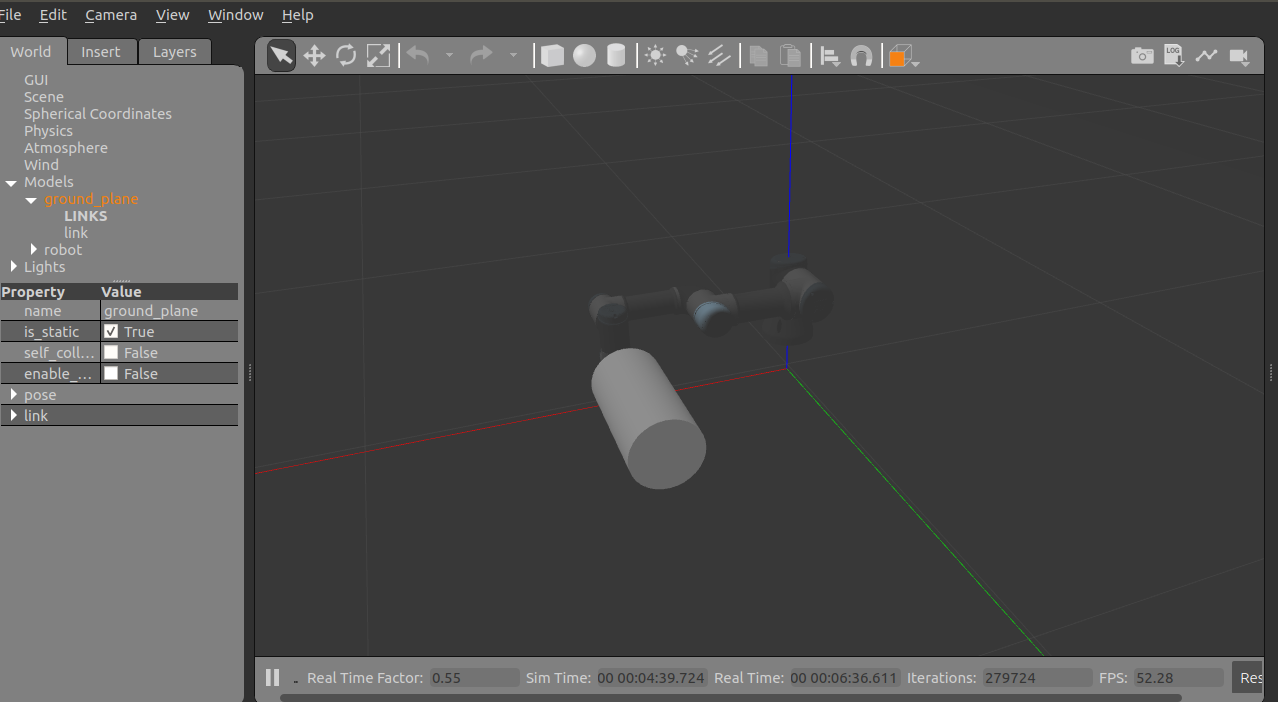
\includegraphics[width=\linewidth]{moveIt_phantom.png}
	\caption{Approximate URDF model of the phantom head.} 
	\label{fig:moveIt_phantom}
\end{figure}

\subsubsection{Virtual joints} Virtual joint attach the robot to the world therefore it is important to define it. Joint type and parent joint must be defined to create a virtual joint.

\subsubsection{Planning groups} Planning groups define the robot kinematic chain semantically and these groups are used later to move the robot. Appropriate kinematic solver has to be defined at this point to let MoveIt know which kinematic solver needs to be used. Popular choices are KDL, universal kinematics, or more powerful IK solver.\\

MoveIt offers many advantages when it comes to commanding the robot such as, 

\begin{enumerate}
	\item \textbf{Getting basic info} basic information such as end-effector position, move group details, planning frame, end-effector link, and joint states can be easily queried using MoveIt.
	\item \textbf{Joint pose goal} robot can be commanded to a specific joint goal by defining an array of joint values.
	\item \textbf{Pose goal} robot can be commanded to a specific pose by defining a homogeneous $4\times4$ pose matrix.
	\item \textbf{Cartesian goal} robot can be commanded to follow a cartesian path by defining a list of waypoints for end-effector to go through.
	\item \textbf{Trajectory display} we can visualize the path planned for the robot via any of the commanding methods.
	\item \textbf{Rviz \& Gazebo simulation} MoveIt seamlessly integrates Rviz and Gazebo simulation to enhance visualization.
\end{enumerate} 